%% ============================================================================
%%  docs/qef_gpu.tex
%%
%%  Caching the QEF: per-frame recomputation versus stored position/normal
%%  in the octree SDF ray marcher.
%%
%%  Impact analysis.  No engine source file is modified by this report.
%% ============================================================================
\documentclass[11pt,a4paper]{article}

\usepackage[T1]{fontenc}
\usepackage[utf8]{inputenc}
\usepackage{lmodern}
\usepackage{microtype}
\usepackage[left=2.4cm,right=2.4cm,top=2.6cm,bottom=2.8cm]{geometry}

\usepackage{amsmath,amssymb,amsthm}
\usepackage{booktabs}
\usepackage{longtable}
\usepackage{array}
\usepackage{tabularx}
\usepackage{float}
\usepackage{caption}
\usepackage{graphicx}
\usepackage{subcaption}
\usepackage{enumitem}
\usepackage{xcolor}
\usepackage{listings}
\usepackage{tcolorbox}
\tcbuselibrary{breakable}
\usepackage{tikz}
\usetikzlibrary{arrows.meta,positioning,shapes.geometric,fit,calc,
                decorations.pathreplacing,backgrounds,patterns}
\usepackage{pgfplots}
\pgfplotsset{compat=1.18}
\usepackage[hidelinks]{hyperref}
\usepackage{url}
\usepackage{cleveref}

\definecolor{evS}{RGB}{20,90,150}
\definecolor{evM}{RGB}{20,130,70}
\definecolor{evR}{RGB}{150,80,20}
\definecolor{evT}{RGB}{110,60,140}
\definecolor{evP}{RGB}{170,40,40}

\newcommand{\evS}{\textsf{\textbf{\color{evS}[S]}}}
\newcommand{\evM}{\textsf{\textbf{\color{evM}[M]}}}
\newcommand{\evR}{\textsf{\textbf{\color{evR}[R]}}}
\newcommand{\evT}{\textsf{\textbf{\color{evT}[T]}}}
\newcommand{\evP}{\textsf{\textbf{\color{evP}[P]}}}

% Paths are breakable (url) so long file:line references do not overrun the
% margin; identifiers stay unbreakable.
\newcommand{\fpath}[1]{\path{#1}}
\newcommand{\code}[1]{\texttt{\detokenize{#1}}}

\newcommand{\dd}{\mathrm{d}}
\newcommand{\vect}[1]{\mathbf{#1}}
\newcommand{\cube}{\mathcal{C}}
\newcommand{\eps}{\varepsilon}

\theoremstyle{plain}
\newtheorem{theorem}{Theorem}
\newtheorem{lemma}{Lemma}
\theoremstyle{definition}
\newtheorem{definition}{Definition}
\theoremstyle{remark}
\newtheorem{remark}{Remark}

\lstdefinestyle{src}{
  basicstyle=\ttfamily\footnotesize,
  keywordstyle=\color{blue!60!black},
  commentstyle=\color{gray!65!black},
  stringstyle=\color{orange!70!black},
  numbers=left,numberstyle=\tiny\color{gray},numbersep=5pt,
  breaklines=true,tabsize=2,showstringspaces=false,
  frame=single,rulecolor=\color{gray!40},
  backgroundcolor=\color{gray!5},
  captionpos=b,
  columns=fullflexible,
  keepspaces=true,
}
\lstset{style=src}

\setlength{\emergencystretch}{3em}
\sloppy
\setlength{\parskip}{2pt}

\title{\textbf{Caching the QEF}\\[6pt]
{\large Per-Frame Recomputation versus Stored Position and Normal\\
in the Octree SDF Ray Marcher}\\[8pt]
{\normalsize An impact analysis}}
\author{Vulkan Engine Technical Report}
\date{\today}

\begin{document}

\maketitle

\begin{abstract}
The octree SDF ray marcher re-solves the dual-contouring QEF for every surface
hit, every frame. The result is a pure function of the eight stored corner
samples and the node cube, so it is constant for a table revision. The raster
terrain path already computes it once per vertex; the raymarch path does not
store it. This report compares the current per-frame recomputation with a
payload that stores the QEF position and normal once, when the node table is
uploaded or derived. The existing \fpath{OctreeDerive.comp} pass already
computes both values for every node while resolving materials and the
Lipschitz bound, and simply discards them. Storing them costs 32\,B/node in an
aligned side buffer (16\,MiB per frame
slot, 48\,MiB for three slots), or 24\,B/node packed (12\,MiB/slot, 36\,MiB
total), and no additional QEF arithmetic. The
fragment then replaces up to four QEF solves, four ring normals and four
terrain material classifications per solid hit with hit-only loads; the
classifier recomputes its own gradient at the QEF position, so a
sentinel-material ring cell currently pays that gradient twice.

At $1280\times720$ and 40\% solid coverage the current path performs about
1.47\,M QEF solves per frame; at 60\,fps that is 169 times as many solves per
second as the one-time pass produces nodes for one slot. At
$3840\times2160$ it is about
13.3\,M per frame and 1519 times per second. The direct FLOP saving is modest relative to
shading at 720p, but the removed divisions, square roots, Perlin-based
material classification, branches and register pressure are concentrated in
the hit path and scale with resolution; at 4K the QEF alone accounts for a
non-trivial fraction of the GPU's arithmetic throughput. The
recommendation is to keep the 96\,B traversal record unchanged, add a separate
32\,B/node (or 24\,B packed) payload written by \fpath{OctreeDerive.comp}, and
consume it only where the stored value is exact: ring positions, ring normals
and cached materials. Analytic normals at the marched hit point remain where
the position differs. The change is a strict improvement for static or
debounced-edit scenes and is exactly invalidated by the existing table
revision.
\end{abstract}

\newpage
\tableofcontents
\newpage

% ============================================================================
\section{Introduction}
% ============================================================================

\subsection{The question}

The engine contains an optional terrain path that replaces rasterized,
tessellated chunks with a fullscreen fragment shader that ray-marches the
octree's stored SDF corner samples
(\fpath{shaders/renderer/octree/OctreeRaymarch.frag}, selected by
\code{Settings::octreeRaymarchEnabled}, default off,
\fpath{types/Settings.hpp:157}). The raster path builds vertices once
(\fpath{shaders/computation/octree/OctreeTriangles.comp}) and stores each
vertex's position, normal, material and mapping payload in a 64-byte GPU
vertex. The raymarch path has no vertex stream: when a ray hits a cell, the
fragment shader reconstructs the cell's surface point and normal on the spot.

The question addressed here is narrow and concrete:
\begin{quote}
What is the impact of calculating the QEF every frame, compared with storing
the position and normal a single time when the node data is loaded into the
GPU?
\end{quote}
The answer is developed from the implementation, not from a synthetic
benchmark. No source file is modified and no measured speed-up is claimed.
Where a number is a static instruction count it is marked as such; where it is
a performance estimate it is labelled as theoretical.

\subsection{Why the QEF, and why now}

A dual-contouring QEF solve is one of the most expensive arithmetic
operations in the hit path: eight analytic corner gradients, up to twelve
edge-plane accumulations, a
regularized $3\times3$ Cramer solve, and a clamp. In the raymarch shader this
work is executed at \emph{hit time}, for the hit cell and for up to four ring
cells around it, on every frame. Yet the inputs---the eight corner SDF values
and the node cube---are immutable between table revisions. The same values are
already computed once per revision by the payload pass
(\fpath{shaders/computation/octree/OctreeDerive.comp}) and then thrown away.
The storage question is therefore not ``compute versus memory'' in the usual
sense: the compute is already being done, and the missing piece is only the
store.

\subsection{Scope and non-goals}

The report analyses:
\begin{itemize}[leftmargin=1.3em,itemsep=1pt]
\item where the QEF is computed in the raster, raymarch and derive paths;
\item how many solves the fragment performs per hit and per frame;
\item the static cost of one solve, measured from the compiled SPIR-V and from
      a standalone optimized probe;
\item the memory, bandwidth and invalidation cost of storing the QEF position
      and normal per node;
\item exactness conditions and the cross-module compilation caveat;
\item the cases in which recomputation is still preferable.
\end{itemize}
It does not analyse traversal algorithms, shading, texture bandwidth or
tessellation displacement beyond their interaction with the QEF. The material
classifier is discussed only because the same payload already caches it; its
accuracy is not evaluated. It also does not propose a new mesh or a new
octree; the existing node table, frame-slot upload and derive pass are
retained.

\subsection{Evidence labels}

The report uses the same five labels as the earlier octree reports.

\begin{center}
\begin{tabular}{@{}ll@{}}
\toprule
Label & Meaning \\
\midrule
\evS & Verified directly in engine source (file and line given). \\
\evM & Measured in a recorded run or a compiled artifact (file/command given). \\
\evR & Reported by external research (citation given). \\
\evT & Theoretical estimate derived in this report; not measured. \\
\evP & Proposal that requires benchmarking before acceptance. \\
\bottomrule
\end{tabular}
\end{center}

The static instruction counts in \cref{sec:cost} were obtained by compiling a
standalone probe that includes \fpath{SdfCell.glsl} with the same
\code{glslc} used by the build, disassembling it with \code{spirv-dis}, and
counting the instructions of the emitted functions. They are compile-time
facts about the module, not GPU cycle measurements. The runtime estimates are
derived from those counts and are labelled \evT.

\subsection{Summary of findings}

\begin{enumerate}[leftmargin=1.4em,itemsep=2pt]
\item \textbf{The per-frame QEF is hit-time work, not traversal work.} The
      material/Lipschitz payload already removed the per-visited-node QEF in
      normal operation. What remains is the ring reconstruction: up to four
      QEF solves, four ring normals and four terrain-material
      classifications per solid hit (\fpath{OctreeRaymarch.frag:442--551}),
      and up to eight
      QEF solves per water pixel because the two water lobes shade two
      secondary solid hits (\fpath{OctreeRaymarch.frag:1246--1374}).
      \evS
\item \textbf{The values are already computed once per revision.}
      \fpath{OctreeDerive.comp:55--57} computes the QEF position, the QEF
      normal and the material for every stored node, then writes only the
      material and Lipschitz bound. Adding the two vectors is two stores in a
      pass that already runs. \evS
\item \textbf{The redundancy is large in aggregate.} At
      $1280\times720$ with 40\% solid coverage the current path solves about
      1.47\,M QEFs per frame; at $3840\times2160$ it is about 13.3\,M per
      frame. The one-time pass computes 524\,288 values per slot. The ratio
      is 2.8:1 per frame and 169:1 per second at 720p, rising to 25.3:1 and
      1519:1 at 4K (per-slot values). \evT
\item \textbf{The direct FLOP saving is resolution-dependent.} At 720p the
      QEF is roughly 1--2\% of the GPU's peak arithmetic throughput; at 4K it
      can be 10--20\% once divisions, square roots and divergence are
      weighted. It is not the dominant cost at 720p, but it is a pure
      redundancy that grows linearly with pixels. \evT
\item \textbf{The ring material classification is an independent, zero-memory
      win.} \code{rmBlendAtHit} calls \code{rmResolveMaterialAt}, which reruns
      the LandBrush classifier and its Perlin fields for each ring cell, even
      though the payload pass already resolved the identical material into
      \code{meta.x}. Reading the cached value removes up to four classifiers
      per hit without any new storage. \evS
\item \textbf{A side buffer is better than growing the record.} Adding the
      payload to the 96\,B record would make every traversal visit fetch 128\,B
      (+33\% traffic on all node visits). A separate 32\,B/node array is read
      only at hits: about 47\,MB/frame at 720p/40\%, versus 590\,MB/frame of
      extra traversal traffic for the in-record variant at 20 visits/ray.
      \evT
\item \textbf{Caching is exact under the revision model.} The QEF position and
      normal are pure functions of the node record, and the whole table is
      rebuilt and re-derived on every revision. There is no partial
      invalidation problem. The only caveat is cross-module floating-point
      determinism, which the existing material cache already depends on and
      which must be verified once. \evS\evT
\item \textbf{Recommendation.} Store the QEF position and normal in a
      per-slot side buffer written by \fpath{OctreeDerive.comp}; use them for
      ring positions, ring normals and cached materials; keep analytic normals
      at the marched hit point. Do not compute the values on the CPU and do
      not grow the traversal record. \evP
\end{enumerate}

% ============================================================================
\section{Where the QEF work happens}
% ============================================================================

\subsection{The solver}

Both the CPU reference and the GPU runtime solve the same regularized
dual-contouring system. For every edge of the cell that changes sign, the
solver interpolates a point $\vect p_i$ and a normal $\vect n_i$ along the
edge, and accumulates
\begin{equation}
A=\sum_i \vect n_i\vect n_i^{\mathsf T},\qquad
\vect b=\sum_i \vect n_i\,(\vect n_i\cdot \vect p_i),\qquad
m=\frac{1}{k}\sum_i \vect p_i .
\label{eq:qef}
\end{equation}
It then pulls the underconstrained solution toward the mass point $m$,
\begin{equation}
(A+0.1\,I)\,\vect x=\vect b+0.1\,m,
\label{eq:reg}
\end{equation}
solves the $3\times3$ system by Cramer's rule, rejects non-finite results, and
clamps the vertex to the cell cube. Exact-zero corners snap to the corner,
infinite sentinels are skipped, and a cell with no usable crossing falls back
to the average of its finite straddling edges. The two implementations are
\fpath{sdf/core/SDF.cpp:6--133} and
\fpath{shaders/includes/octree/SdfCell.glsl:125--232}; the shader is a
deliberate port of the CPU function with \code{precise} qualifiers and the
dot/length/outer-product operations spelled out in the same order
(\fpath{SdfCell.glsl:16--22}). \evS

The shader also provides the analytic trilinear gradient used for normals
(\fpath{SdfCell.glsl:69--98}):
\begin{equation}
\nabla f(\vect p)=
\frac{1}{h}\Bigl(\partial_x f,\partial_y f,\partial_z f\Bigr),
\label{eq:grad}
\end{equation}
normalized with a $10^{-6}$ fallback. One QEF solve calls this gradient eight
times, once per corner, and the material path calls it once more at the QEF
position.

\subsection{Three consumers of the same values}

\begin{table}[t]
\centering
\small
\caption{Where the QEF position and normal are computed in the current
engine. The derive pass is the only place that computes them once per node.}
\label{tab:consumers}
\begin{tabularx}{\linewidth}{@{}lXl@{}}
\toprule
Path & Where and when & Stored? \\
\midrule
Raster topology
  & \code{writeVertexOnce} during chunk build, per referenced vertex
  & yes, 64\,B vertex \\
Raymarch march material
  & \code{rmResolvedBrush} on a visited node, only if payload absent
  & material only (\code{meta.x}) \\
Raymarch hit ring
  & \code{rmBlendAtHit}, up to four ring cells, every frame
  & \textbf{no} \\
Raymarch water lobes
  & \code{rmShadeSolidHit} for refraction and reflection, every frame
  & \textbf{no} \\
Derive pass
  & \code{OctreeDerive.comp}, once per revision per slot, every node
  & material/Lipschitz only; QEF/normal discarded \\
\bottomrule
\end{tabularx}
\end{table}

\paragraph{Raster path: once per vertex.}
\fpath{shaders/computation/octree/OctreeTriangles.comp:985--1011} calls
\code{cellPos(c)} and \code{cellNormal(c,p)} once for each referenced surface
node, resolves the terrain material, and writes the 64-byte vertex payload
(\fpath{OctreeTriangles.comp:956--980}). The position may already be the
feature-refined QEF result produced by
\fpath{shaders/computation/octree/OctreeVirtualRefine.comp}
(\fpath{OctreeTriangles.comp:274--289}). This is exactly the ``store once''
strategy: the cost is paid at mesh-build time and the fragment interpolates.
\evS

The raster vertex pools are not a drop-in source for the raymarch. They are
chunk-local, they only cover nodes that received a vertex slot, and they can
be rebuilt or evicted independently of the raymarch table. The raymarch table
includes all stored surface nodes, including coarse parents and pruned
fallbacks, and it is uploaded as a separate whole-scene structure. Coupling
the two paths would add a second indirection and a lifetime dependency. The
node-local payload described here is the raymarch analogue of the raster
vertex payload, at node rather than vertex granularity. \evS

\paragraph{Raymarch path: once per hit, every frame.}
The march itself does not solve the QEF per visited node in normal operation:
\code{rmCachedBrush} reads the derived material from \code{meta.x} when
\code{RM_FLAG_PAYLOAD} is set (\fpath{OctreeRaymarch.frag:196--223}). The QEF
survives in the hit reconstruction:
\begin{itemize}[leftmargin=1.3em,itemsep=1pt]
\item \code{rmBlendAtHit} reconstructs the raster TCS's three-material
      triangle for the hit cell. For each of the four quadrant cells it calls
      \code{rmCellQef(id)} (\fpath{OctreeRaymarch.frag:528}), classifies the
      material with \code{rmResolveMaterialAt(id,qp)}
      (\fpath{OctreeRaymarch.frag:538}) and computes the normal with
      \code{rmNodeNormal(id,qp)} (\fpath{OctreeRaymarch.frag:539}). For a
      \code{LAND_BRUSH_INDEX} or \code{NORMAL_BRUSH} cell the classifier
      internally computes \code{sdfCellNormal} at \code{qp} to feed its slope
      test (\fpath{OctreeRaymarch.frag:171--181}); that is the same gradient
      the next line computes again for the ring normal. The cached material
      removes the first copy; the cached normal removes the second.
\item \code{rmResolveHitShading} calls \code{rmNodeNormal} at the hit point
      and, when tessellation displacement is active, at up to two fixed-point
      base points (\fpath{OctreeRaymarch.frag:1026--1059}). These are
      gradients, not QEF solves; they are not exactly the stored QEF normal
      because the position differs.
\item The water branch with RT shading off calls \code{rmShadeSolidHit} for
      the refracted lake bed and for the mirror reflection
      (\fpath{OctreeRaymarch.frag:1272--1374}). Each of those is a full solid
      hit and therefore another ring reconstruction with up to four QEF
      solves. A water pixel can therefore trigger up to eight QEF solves
      before its own shading, while its own water normal is only one
      gradient (\fpath{OctreeRaymarch.frag:1462}). \evS
\end{itemize}

\paragraph{Derive path: once per revision, values discarded.}
\fpath{shaders/computation/octree/OctreeDerive.comp:43--65} runs one
invocation per stored node and computes:
\begin{lstlisting}[language=C++,float=t,caption={The derive pass already computes the exact values this report proposes to store.}]
float sdf[8];
for (int c = 0; c < 8; ++c) sdf[c] = ...;
vec3 mn = nodes[i].cubeMinSize.xyz;
float sz = nodes[i].cubeMinSize.w;

vec3 qef = sdfCellPosition(sdf, mn, sz);
vec3 n   = sdfCellNormal(sdf, mn, sz, qef);
int  mat = rmResolveMaterialAtCorners(int(nodes[i].meta.z), sdf, mn, sz, qef, n);
float lip = rmLipBound(sdf, sz);

nodes[i].meta.x = mat;
nodes[i].hsv1.z = 1.0 / max(lip, 1e-3);
nodes[i].meta.w |= int(RM_FLAG_PAYLOAD);
\end{lstlisting}
The pass exists to cache the material and the Lipschitz bound in the record's
previously dead bytes (\fpath{OctreeDerive.comp:3--19}). It computes the QEF
position and normal to feed the classifier, then writes neither. \evS

\subsection{Data flow}

\begin{figure}[t]
\centering
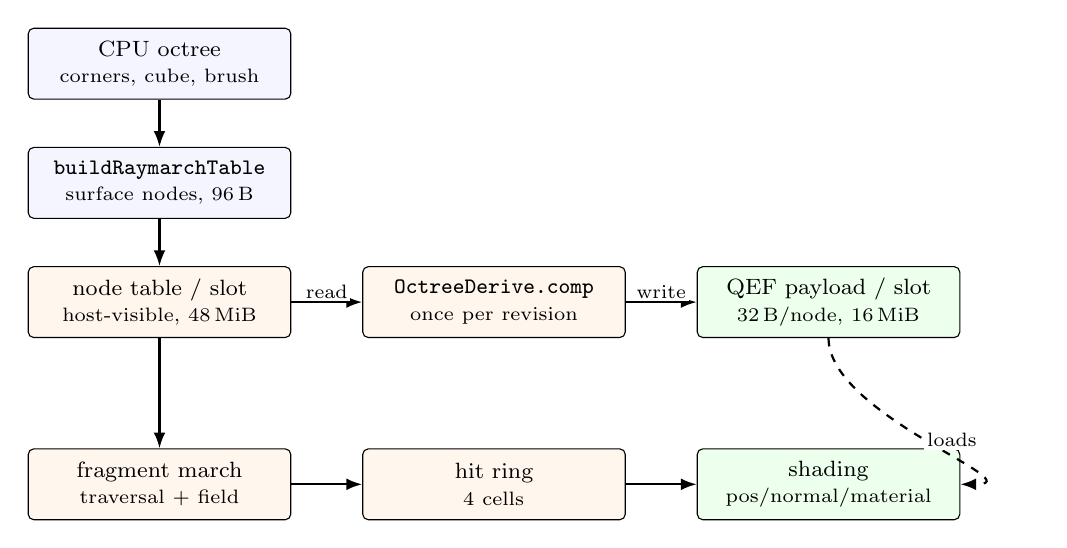
\begin{tikzpicture}[
  node distance=6mm and 9mm,
  box/.style={draw,rounded corners=2pt,align=center,font=\footnotesize,
              minimum height=9mm,text width=31mm,fill=blue!4},
  gpu/.style={box,fill=orange!7},
  pay/.style={box,fill=green!7},
  arr/.style={-{Latex[length=2mm]},thick},
  lbl/.style={font=\scriptsize,fill=white,inner sep=1pt}
]
\node[box] (cpu) {CPU octree\\\scriptsize corners, cube, brush};
\node[box,below=of cpu] (build) {\code{buildRaymarchTable}\\ \scriptsize surface nodes, 96\,B};
\node[gpu,below=of build] (table) {node table / slot\\ \scriptsize host-visible, 48\,MiB};
\node[gpu,right=of table] (derive) {\code{OctreeDerive.comp}\\ \scriptsize once per revision};
\node[pay,right=of derive] (payload) {QEF payload / slot\\ \scriptsize 32\,B/node, 16\,MiB};
\node[gpu,below=14mm of table] (march) {fragment march\\ \scriptsize traversal + field};
\node[gpu,right=of march] (ring) {hit ring\\ \scriptsize 4 cells};
\node[pay,right=of ring] (shade) {shading\\ \scriptsize pos/normal/material};

\draw[arr] (cpu) -- (build);
\draw[arr] (build) -- (table);
\draw[arr] (table) -- node[lbl,above]{read} (derive);
\draw[arr] (derive) -- node[lbl,above]{write} (payload);
\draw[arr] (table) -- (march);
\draw[arr] (march) -- (ring);
\draw[arr] (ring) -- (shade);
\draw[arr,dashed] (payload.south) to[out=-90,in=0] node[lbl,right]{loads} (shade.east);
\end{tikzpicture}
\caption{The proposed data flow. The derive pass reads the same 96\,B node
records the march uses and writes a parallel, hit-only QEF payload. The march
itself is unchanged; only the hit ring reads the payload instead of solving.}
\label{fig:flow}
\end{figure}

The important property of \cref{fig:flow} is that the payload is a sibling of
the node table, not a replacement for any field. The traversal record stays at
96\,B and the march's field evaluation is untouched. The only new dependency
is \code{COMPUTE_SHADER_WRITE -> FRAGMENT_SHADER_READ} on the payload
buffer, which the existing derive barrier can cover.

\subsection{Revision model}

The table is rebuilt breadth-first by \code{LocalScene::buildRaymarchTable}
(\fpath{utils/LocalScene.cpp:498--683}) and uploaded into the frame slot when
its revision changes (\fpath{vulkan/renderer/octree/OctreeRaymarchRenderer.cpp:284--312}).
Rebuilds are debounced by 0.4\,s (\fpath{MyApp.cpp:4776}) except after a
brush stroke, where the timer is set past the threshold so the next frame
rebuilds (\fpath{MyApp.cpp:5271}). Node indices are only stable within one
revision. This is precisely the granularity at which the QEF position and
normal are constant. \evS

% ============================================================================
\section{The cost of one solve}
\label{sec:cost}
% ============================================================================

\subsection{Source-level cost}

The CPU/GLSL solver performs the following work for a surface cell:
\begin{itemize}[leftmargin=1.3em,itemsep=1pt]
\item eight corner gradients, each a trilinear gradient with a normalization;
\item a loop over the twelve cell edges, with the expensive accumulation only
      on sign-changing edges (typically three to six);
\item a regularized $3\times3$ solve: four $3\times3$ determinants and three
      divisions;
\item fallback averaging, non-finite guards and a final clamp.
\end{itemize}
A source-level operation count gives roughly 700--1200 floating-point
operations, 11--23 divisions and 12--20 square roots per solve, depending on
the number of crossings and the corner specialization. The earlier octree
report used $\approx 940$ FLOP as a representative estimate
\cite{raymarchReport}. This is a useful bound but it overstates
the compiled corner gradients: at a cell corner the local coordinates are
exactly 0 or 1, so most of the trilinear weights vanish. The compiler can
specialize each of the eight calls. \evT

\subsection{Compiled evidence}

To get a concrete static count we compiled two probes with the engine's
\code{glslc} and counted the emitted SPIR-V instructions. The first probe is
the actual per-frame module, \fpath{bin/shaders/renderer/octree/OctreeRaymarch.frag.spv};
the second is a standalone compute shader that includes the same
\fpath{SdfCell.glsl} and calls \code{sdfCellPosition} and
\code{sdfCellNormal} once on runtime values. The build compiles the raymarch
fragment \emph{without} \code{-O} (the generic rule at
\fpath{Makefile:294--302} passes an empty optimization argument; only selected
water modules use \code{GLSL_OPT}), so the shipped module preserves the
function structure. The driver still optimizes at ISA generation time, but the
module itself is unoptimized.

\begin{table}[t]
\centering
\small
\caption{Static SPIR-V instruction counts. ``Arith'' counts arithmetic
instructions (`OpFAdd`, `OpFSub`, `OpFMul`, `OpFDiv`, `OpVectorTimesScalar`,
`OpMatrixTimesVector`) and therefore includes divisions; ``ext'' counts
`OpExtInst` (sqrt, abs, clamp). ``L/S'' counts `OpLoad`/`OpStore`. The shipped
fragment is unoptimized; the probe is shown both unoptimized and with
\code{-O}. ``Total'' counts every instruction in the function body, including
call setup, composite construction and control flow, so it exceeds the sum of
the listed columns. Counts are static module instructions, not executed
cycles.}
\label{tab:spirv}
\begin{tabularx}{\linewidth}{@{}lrrrrr@{}}
\toprule
Module & Arith & Ext & L/S & Branches & Total \\
\midrule
\code{sdfCellPosition} (shipped, unoptimized) & 53 & 6 & 224 & 23 & 633 \\
\code{sdfCellNormal} (shipped, unoptimized) & 66 & 1 & 88 & 1 & 227 \\
\code{sdfCellPosition} (probe, \code{-O}) & 257 & 2 & 34 & -- & -- \\
\code{sdfCellNormal} (probe, \code{-O}) & 65 & 1 & 8 & -- & -- \\
QEF + one normal (probe, \code{-O}) & 322 & 3 & 42 & -- & -- \\
\bottomrule
\end{tabularx}
\end{table}

The shipped \code{sdfCellPosition} is not a small inline sequence: it contains
the eight-corner loop and calls \code{sdfCellNormal} from inside it, so one
dynamic solve executes the body of \code{sdfCellNormal} eight times. The
optimized probe shows what the arithmetic reduces to once the corner
specialization and common subexpressions are folded: about 257 arithmetic
instructions (23 of them divisions) and 2 square roots for the
QEF, plus 65 arithmetic instructions (9 of them divisions) and 1 square root
for one general normal. The combined figure is 322 arithmetic instructions,
32 of them divisions, plus 3 square roots for the QEF and one ring normal. A
sentinel-material cell pays one more normal for the classifier (65
arithmetic instructions, 9 of them divisions, 1 square root), which the
cached material also removes. \evS\evM

\paragraph{What the counts do not include.}
The counts exclude branch divergence, memory latency, instruction-cache
pressure and the material classifier. They also exclude the driver's own
optimization, which can lower the arithmetic but cannot remove the
data-dependent branches around the edge loop. They are therefore best read as
a relative weight, not an absolute cycle count.

\subsection{The material classifier}

For a ring cell painted with \code{LAND_BRUSH_INDEX} (255) or
\code{NORMAL_BRUSH} (254), \code{rmResolveMaterialAt} computes a gradient at
the QEF position and calls the classifier. For terrain, the classifier is not
a small lookup: \code{landMaterialIndex} selects a rock or grass biome and
runs \code{landBiomeShape}, which evaluates three 2D Perlin fields
(\fpath{shaders/includes/octree/LandBrush.glsl:44--49,126--169};
\fpath{shaders/includes/noise/Perlin2D.glsl:41--54}). Each Perlin evaluation
hashes four lattice gradients, four dot products, a fade and three mixes.
Three Perlin fields per classifier, four ring cells per hit, means up to
twelve noise evaluations per solid hit. \evS

This is the same value that \code{OctreeDerive.comp} already resolved into
\code{meta.x}, and the ring path does not use it. The material cache is
therefore an independent optimization: it costs no memory and removes a
branchy, noise-heavy computation from the per-pixel path. It should be taken
whether or not the QEF payload is implemented.

% ============================================================================
\section{How much QEF work is done per frame}
% ============================================================================

\subsection{Counts per hit}

Let $q_s=4$ be the maximum number of ring cells for a solid hit and $q_w=8$
the maximum for a water pixel with two secondary solid hits. The primary
raymarch path then performs
\begin{equation}
Q_{\text{frame}} = q_s\,h\,P + q_w\,w\,P,
\label{eq:qframe}
\end{equation}
QEF solves per frame, where $P=W H$ is the pixel count, $h$ the solid-hit
fraction and $w$ the water-hit fraction with RT shading off. The ring is
``up to four'' because duplicate/absent quadrants are dropped
(\fpath{OctreeRaymarch.frag:517--551}); four is the normal upper bound for a
terrain cell.

The same formula in terms of the node count $N$ is more revealing. The
one-time derive pass computes $N$ values per slot; the per-frame path computes
$Q_{\text{frame}}$, and the per-second multiplier at $f$ frames per second is
$fQ_{\text{frame}}/N$. At $N=524\,288$ (the node cap,
\fpath{OctreeRaymarchRenderer.hpp:41--48}):

\begin{table}[H]
\centering
\small
\caption{Per-frame QEF solves for solid-only terrain at 40\% coverage
($q_s=4$), and the ratio to the one-time 524\,288-node derive for one slot.
The per-second column is at 60\,fps.}
\label{tab:qframe}
\begin{tabular}{@{}lrrrr@{}}
\toprule
Resolution & Pixels & QEF/frame & QEF/s at 60\,fps & Ratio/s \\
\midrule
$1280\times720$   & 921\,600  & 1.474\,M & 88.5\,M  & $169\times$ \\
$1920\times1080$  & 2\,073\,600 & 3.318\,M & 199.1\,M & $380\times$ \\
$2560\times1440$  & 3\,686\,400 & 5.898\,M & 353.9\,M & $675\times$ \\
$3840\times2160$  & 8\,294\,400 & 13.27\,M & 796.3\,M & $1519\times$ \\
\bottomrule
\end{tabular}
\end{table}

The table is deliberately simple: it uses the maximum of four ring cells per
hit and 40\% coverage, and ignores the water secondary hits. For a 40\% solid
view these are upper bounds (duplicate quadrants reduce the ring count). With
10\% water coverage the 720p count rises from 1.47\,M to 2.21\,M per frame,
because each water pixel adds eight solves. The per-frame count is 2.8 times
the number of node values per slot at 720p and
25 times at 4K; the per-second count is two to three orders of magnitude
larger. That is the redundancy the cache removes. \evT

The derive pass runs once per frame slot, so a revision actually computes
$3N=1\,572\,864$ values. The ratios in the table are per slot, i.e.\ the values
one frame consumes; against the full three-slot revision the ratios are three
times smaller: $0.94{:}1$ per frame and $56{:}1$ per second at 720p, and
$8.4{:}1$ and $506{:}1$ at 4K. The per-slot framing is the relevant one for a
frame; the full-revision figure is also why a revision-shared payload is
worth considering later. \evT

\subsection{Arithmetic volume}

Multiplying by the optimized per-ring-cell counts (322 arithmetic, 32
divisions, 3 square roots) gives the arithmetic volume in
\cref{tab:arith}. The table separates the solid-only case at 40\% coverage;
the water case is additive.

\begin{table}[H]
\centering
\small
\caption{Arithmetic volume of the per-frame QEF ring work, from
\cref{tab:qframe} and the optimized probe counts. ``ALU'' counts the
arithmetic instructions and includes the divisions shown in the next column;
square roots are listed separately. The final column is the ALU rate at
60\,fps. These are static instruction volumes, not measured GPU throughput.}
\label{tab:arith}
\begin{tabular}{@{}lrrrr@{}}
\toprule
Resolution & ALU/frame & Div/frame & Sqrt/frame & ALU/s at 60\,fps \\
\midrule
$1280\times720$  & 474.5\,M & 47.2\,M & 4.4\,M & 28.5\,G \\
$1920\times1080$ & 1.068\,G & 106.2\,M & 9.9\,M & 64.1\,G \\
$2560\times1440$ & 1.899\,G & 188.7\,M & 17.7\,M & 113.9\,G \\
$3840\times2160$ & 4.273\,G & 424.7\,M & 39.8\,M & 256.4\,G \\
\bottomrule
\end{tabular}
\end{table}

Because the static counts include both sides of the QEF branches, the volumes
in the table are upper bounds on the executed arithmetic; the dynamic count is
lower, and only the proposed counters can measure it. The table uses the
QEF-plus-one-normal figure. A \code{LAND} ring cell pays
one additional classifier normal (65 arithmetic, 9 divisions, 1 square root)
before the material is known, so the true terrain volume is about 20\% higher
from that normal alone, before the Perlin fields; the cached-material variant
removes both the extra normal and the noise, and the table's figures then
apply. \evT

On a reference integrated GPU with roughly 3.4\,TFLOP/s peak FP32, the 720p
ALU rate is below 1\% of peak; the 4K rate is about 7.5\% before division and
square-root weighting. Divisions are much slower than multiplies on current
GPUs (often one quarter to one eighth rate), and square roots are slower
still. Weighting a division as four ALU operations and a square root as eight
raises the 4K figure to roughly 10--14\% of peak, before divergence. At 720p
the same weighting gives about 1--2\%. These are order-of-magnitude estimates,
not measurements. \evT

\subsection{Why the arithmetic share is not the whole story}

Four effects make the runtime cost larger than the FLOP count suggests.

\begin{enumerate}[leftmargin=1.4em,itemsep=2pt]
\item \textbf{Divergence.} The ring loop runs for hit pixels but not for miss
      pixels. Within a wave, some lanes may have hit and others not; the
      lanes that hit execute the QEF while the others wait. The four ring
      cells also have different validity and different sign patterns, so the
      edge loop's branches diverge within a single hit. A FLOP count assumes
      perfect SIMD utilization; the QEF path does not have it.
\item \textbf{Register pressure.} The solver holds eight corner normals (24
      floats), a $3\times3$ matrix (9 floats), the mass point and the
      accumulator, plus the edge temporaries. Even when only hit lanes execute
      it, the compiler must allocate registers for the worst-case path of the
      shader. High VGPR usage reduces occupancy for every fragment, including
      misses. Removing the solver from the fragment module can therefore
      improve latency hiding for the whole pass, not just for hits.
\item \textbf{Special-function throughput.} The solver issues divisions and
      square roots in a dependent chain (normalize corner, mix, normalize
      edge, solve). Their throughput is a fraction of FMA throughput, and
      their latency is exposed when the ring cells are processed serially.
\item \textbf{Instruction footprint.} The base fragment is a 371\,KB SPIR-V
      module with the QEF kept as a function; compiling it with \code{-O}
      inlines the march and produces a 6.4\,MB module, which is why the build
      does not optimize it. The QEF code is a non-trivial part of that
      footprint. Moving it to a compute pass keeps the fragment's instruction
      cache focused on traversal and shading.
\end{enumerate}

The combination explains why a change that looks like ``a few hundred FLOPs''
can still be worth several percent of a hit-heavy pass, especially at 4K.

% ============================================================================
\section{What storing the values costs}
% ============================================================================

\subsection{What needs to be stored}

The derive pass already computes and stores the material in \code{meta.x}
and the inverse Lipschitz bound in \code{hsv1.z}; both are existing 4\,B
fields, so they add no record memory. The missing values are:
\begin{itemize}[leftmargin=1.3em,itemsep=1pt]
\item the QEF position, three floats (12\,B);
\item the QEF normal, three floats (12\,B), or an octahedral pair (4\,B).
\end{itemize}
A full-precision position and normal is 24\,B/node. A 32\,B aligned record
(two \code{vec4}s) is the natural GPU layout: one 32\,B sector per access, no
straddling, and a clean std430 array. The 24\,B packed form saves 25\% memory
but can straddle sectors and is not worth the complexity unless memory is
tight.

\subsection{Layout options}

\begin{table}[t]
\centering
\small
\caption{Storage options at the 524\,288-node cap and three frames in flight.
``Traversal'' is the bytes read per visited node; the payload is read only at
hits. Exactness of each variant is discussed in \cref{sec:exact}.}
\label{tab:layouts}
\begin{tabularx}{\linewidth}{@{}lrrrrX@{}}
\toprule
Option & B/node & MiB/slot & MiB total & Traversal & Notes \\
\midrule
Current record & 96 & 48.0 & 144.0 & 96\,B & baseline \\
Side, packed & 24 & 12.0 & 36.0 & 96\,B & exact, may straddle \\
Side, aligned & 32 & 16.0 & 48.0 & 96\,B & exact, recommended \\
Position only & 12/16 & 6.0/8.0 & 18.0/24.0 & 96\,B & normal still solved \\
In-record, packed normal & 112 & 56.0 & 168.0 & 112\,B & exact position, quantized normal \\
In-record, full & 128 & 64.0 & 192.0 & 128\,B & exact, worst traffic \\
Compressed side & 12 & 6.0 & 18.0 & 96\,B & not bit-exact \\
\bottomrule
\end{tabularx}
\end{table}

The in-record variants are included because they are the obvious first
thought: the record has six \code{vec4}s; adding a seventh and eighth is easy.
They are the wrong trade. The QEF payload is needed only at hits, while every
node visit pays for the larger stride. The side buffer keeps the traversal
working set at 96\,B and pays the extra bytes only when a ring cell is
actually reconstructed.

\subsection{Memory arithmetic}

The node table at the cap is
\begin{equation}
96\,\text{B}\times 524\,288 = 48.0\,\text{MiB per slot},\qquad
3\times 48.0 = 144.0\,\text{MiB}.
\end{equation}
A 32\,B side payload adds
\begin{equation}
32\,\text{B}\times 524\,288 = 16.0\,\text{MiB per slot},\qquad
3\times 16.0 = 48.0\,\text{MiB},
\end{equation}
for a total of 192\,MiB: exactly the footprint of the old 128\,B record, but
with the traversal stride still 96\,B. The packed 24\,B version totals
180\,MiB. These figures assume the cap is reached; the earlier octree report
measured the reference scene at the cap, and larger scenes are truncated to
it \cite{raymarchReport}. \evS\evT

If the payload buffer is shared across the three slots instead of copied, the
total drops to 16\,MiB (aligned), but that requires a revision-aware lifetime
so a slot cannot derive the next revision while another slot still reads the
previous one. Per-slot buffers are simpler and match the existing node-table
lifetime; the 32\,MiB saving is not worth a new synchronization problem in the
first implementation.

\subsection{Per-frame bandwidth}

At a hit, the ring reads one payload entry per unique ring cell. With the
aligned layout that is $4\times32=128$\,B per solid hit; with the packed
layout $4\times24=96$\,B. At 720p and 40\% coverage:
\begin{equation}
368\,640\text{ hits}\times128\,\text{B}=47.2\,\text{MB/frame},\qquad
\times60=2.8\,\text{GB/s}.
\end{equation}
The packed form gives 35.4\,MB/frame and 2.1\,GB/s. On the reference APU's
unified memory this is a few percent of the available bandwidth; on a
discrete GPU it is far below the link budget. Adjacent pixels share ring
cells, so the L1/L2 hit rate is high and the effective traffic is lower.

Compare that with growing the record. A moderate terrain ray visits about 20
nodes (the earlier report's profile; grazing rays visit more, sky rays fewer).
At 20 visits per ray and 921\,600 rays:
\begin{equation}
18.43\text{M visits}\times32\,\text{B}=590\,\text{MB/frame},\qquad
\times60=35.4\,\text{GB/s}.
\end{equation}
That is 12--17 times the side-buffer traffic, and it is paid by every ray,
including misses. On a 50\,GB/s APU it would consume most of the bandwidth
before any shading. This is the decisive argument for the side buffer.
\evT

\subsection{Derive cost}

The derive pass already runs once per revision per frame slot. Adding two
\code{vec4} stores per node costs 16\,MiB of writes per slot, 48\,MiB per
revision for three slots; at 50\,GB/s that is roughly 1\,ms, on top of a pass
that already computes the QEF, the normal, the classifier and the Lipschitz
bound. The QEF arithmetic is unchanged. The pass is therefore the ideal
producer: the values are already in registers, and the only new work is the
store. \evT

The CPU alternative is worse. \code{buildRaymarchTable} would have to call
\code{SDF::getPosition} and \code{SDF::getNormalFromPosition} for every stored
node: about $0.4$--$0.7$\,GFLOP plus several million divisions and square
roots, single-threaded in the current build path. Even parallelized across
eight threads it adds tens of milliseconds to a rebuild and another 36--48\,MiB
of host-to-device traffic. The GPU already computes the same values in the
derive pass. \evT

\subsection{Derive amortization}

Let $T_d$ be the extra derive time per revision (all three slots) and $S$ the
per-frame time saved. The cache pays back after $F=T_d/S$ frames. With
$T_d\approx3$\,ms:
\begin{center}
\begin{tabular}{@{}lrrrr@{}}
\toprule
$S$ (ms/frame) & 0.2 & 0.5 & 1.0 & 2.0 \\
\midrule
Break-even frames & 15 & 6 & 3 & 2 \\
Break-even time at 60\,fps & 0.25\,s & 0.10\,s & 0.05\,s & 0.03\,s \\
\bottomrule
\end{tabular}
\end{center}
The table is intentionally pessimistic: it charges the full derive cost to a
single frame. In practice the table is static between edits, so the cost is
amortized over thousands of frames. With the 0.4\,s debounce, even continuous
painting issues at most 2.5 revisions per second, i.e.\ 7.5\,ms/s of derive
overhead, which is below one percent of a 60\,fps budget. \evT

% ============================================================================
\section{Correctness and invalidation}
\label{sec:exact}
% ============================================================================

\subsection{The purity lemma}

\begin{lemma}[QEF payload validity]
\label{lem:pure}
For a fixed node record $N$ (eight corner samples and cube), the QEF position
$p_N$ and the QEF normal $n_N$ produced by \code{sdfCellPosition} and
\code{sdfCellNormal} are constants. They change only when the record changes,
i.e.\ when the table revision changes.
\end{lemma}
\begin{proof}
The solver reads only the eight corner values stored in \code{sdf0}/\code{sdf1}
and the cube stored in \code{cubeMinSize}; the edge table, the 0.1
regularization and the fallback constants are compile-time constants. The
algorithm has no time, frame, camera or ray input. Therefore the outputs are
a deterministic function of the record. The table builder is the only writer
of the corner and cube fields, and it rewrites the whole table on a revision.
The derive pass writes the derived fields for every record of that revision
before the march reads it, or leaves the payload flag clear if it cannot run.
\end{proof}

The existing \code{RM_FLAG_PAYLOAD} contract already relies on this lemma for
the material and the Lipschitz bound. Extending the payload to the QEF
position and normal adds no new invalidation source. The whole-table revision
is the generation; there is no partial update, no per-node version and no
address reuse issue. If incremental table updates are added later, the
payload must be updated for every touched node, exactly like the material.

\subsection{Cross-module determinism}

The derive shader and the fragment shader include the same
\fpath{SdfCell.glsl} and call the same functions. The GLSL source is written
to be bit-exact to the CPU port: \code{precise} on the sensitive expressions,
and dot/length/outer-product spelled out in the same order
(\fpath{SdfCell.glsl:16--22}). Bit-exactness across two separately compiled
modules is not guaranteed by the GLSL specification, however. The existing
material cache already has this property: \code{meta.x} is produced by the
derive module and consumed by the fragment, and the fallback path computes the
same classifier in the fragment module. The engine accepts that risk today.

For the QEF payload the risk is slightly larger because the ring geometry and
the barycentric weights depend on the position. The recommended verification
is a one-time debug comparison: for a sample of nodes, recompute the QEF in a
fragment/compute variant and compare the bit patterns with the stored payload;
report the maximum ULP difference and the number of differing nodes. If the
difference is zero on the target compiler, the cached path is bit-identical.
If it is a few ULPs, document the tolerance and verify with an image diff; the
near-singular cells are exactly the ones the \code{precise} qualifiers were
added for, so the difference should be rare and sub-visible. Do not quantize
the position before this test; quantization turns ``maybe a few ULPs'' into a
guaranteed deviation. \evS\evT

\subsection{Edge cases}

\begin{itemize}[leftmargin=1.3em,itemsep=2pt]
\item \textbf{Exact-zero corner snap.} The solver returns the corner before
      any gradient work. The stored value is that corner; the fragment would
      return the same. \evS
\item \textbf{Infinite sentinels and no-crossing fallback.} The solver skips
      non-finite corners and averages finite straddling edges. The stored
      value is the result of the same branches; there is no special case at
      the consumer. \evS
\item \textbf{Clamp and non-finite guards.} The stored position is already
      clamped and guarded by the producer; the consumer does not need to
      repeat the clamp. \evS
\item \textbf{Non-surface and pruned nodes.} The table stores surface nodes
      only; pruned surface children fall back to the parent's field and the
      parent record, which has a payload. There is no record to load for a
      child that was never stored. \evS
\item \textbf{Water layer.} Water nodes are stored and derived like solid
      nodes. The water shading uses the analytic normal at the hit point, not
      the stored QEF normal, so storing the payload does not change the water
      interface normal. The water lobes' secondary solid hits use the payload
      exactly like any solid hit. \evS
\item \textbf{Tessellation displacement.} The ring uses the undisplaced QEF
      position and its normal, then applies the material's displacement; this
      is what the current code does. \code{rmResolveHitShading} keeps its
      analytic normals at the displaced hit/base points, because those
      positions differ from the QEF vertex. \evS
\item \textbf{Derive unavailable.} If the compute pipeline or module is
      missing, the flag is never set and the fragment falls back to the
      current solver. The payload buffer is never read. This is the existing
      behavior for the material payload and should be preserved. \evS
\item \textbf{Empty table.} No draw, no payload; the renderer already handles
      \code{rootCounts_ == 0}. \evS
\end{itemize}

\subsection{Precision of compressed variants}

A 12\,B compressed payload would store the position as three 16-bit unorm
offsets inside the cell and the normal as an octahedral 16-bit pair. For a
30-unit cell the position quantization step is
\begin{equation}
\Delta = \frac{30}{65535} \approx 4.6\times10^{-4}\,\text{units},
\end{equation}
about 130 times below the 0.06-unit hit epsilon. The normal error is
sub-milliradian. Visually this is negligible, and the material thresholds
(steepness 0.980/0.985) are broad enough that a flip would be rare. It is
still not bit-identical, and the ring barycentrics would shift by a tiny
amount. Use full fp32 for the parity path; compression is a later
memory-optimization experiment, not the first implementation. \evT

\subsection{Synchronization and Vulkan details}

The existing sequence in \code{OctreeRaymarchRenderer::recordDerive} is:
\begin{enumerate}[leftmargin=1.4em,itemsep=1pt]
\item a \code{HOST -> COMPUTE} barrier publishing the mapped node-table
      rewrite;
\item the derive dispatch;
\item a \code{COMPUTE -> FRAGMENT} barrier publishing the derived fields
      before the march.
\end{enumerate}
A payload buffer written by the same dispatch is covered by the same
\code{COMPUTE_SHADER_WRITE -> FRAGMENT_SHADER_READ} memory barrier; no
extra barrier is required. The descriptor set gains one storage-buffer
binding (set 2, binding 2) with \code{COMPUTE | FRAGMENT} stage flags, and the
descriptor pool grows from two to three storage buffers per set; both the
compute and graphics pipeline layouts must include the new binding. The
buffer is device-local and written only by the GPU; the CPU never maps it.
The node table remains host-visible and persistently mapped. If a CPU-filled
fallback is ever added, it needs its own \code{HOST -> FRAGMENT} barrier, but
that is not the recommended path. \evS

The buffer range must cover \code{maxNodes * stride}. The existing
\code{maxNodes_} is computed from the device's storage-buffer range and
\code{sizeof(OctreeRaymarchNode)}; the payload allocation should take the
minimum of that bound and \code{maxStorageBufferRange / 32}. On a device with
a small storage-buffer range, the payload and node table caps must agree, or
the derive dispatch could write past the payload. \evS

% ============================================================================
\section{Impact comparison}
% ============================================================================

\subsection{Variants}

\begin{table}[H]
\centering
\footnotesize
\caption{The practical variants. ``Ring work'' is per solid hit. ``Exact''
means bit-identical to the current image on the target compiler, subject to
\cref{sec:exact}.}
\label{tab:variants}
\begin{tabularx}{\linewidth}{@{}lXrrX@{}}
\toprule
Variant & Ring work per solid hit & Extra memory & Exact & Verdict \\
\midrule
A. Current
  & 4 QEF + 4 normals + 4 classifiers
  & 0 & -- & baseline \\
B. Cached material only
  & 4 QEF + 4 normals + 4 reads
  & 0 & yes & do first \\
C. B + position
  & 4 loads + 4 normals + 4 reads
  & 18/24\,MiB & yes & good if memory-tight \\
D. B + position + normal
  & 8 loads + 4 reads
  & 36/48\,MiB & yes & recommended \\
E. D + stored normal at hit point
  & fewer gradients
  & same & approximate & phase 2 \\
F. In-record 128\,B
  & same as D
  & 48\,MiB + 33\% traversal & yes & avoid \\
G. CPU compute at build
  & same as D
  & build time + upload & yes & avoid \\
\bottomrule
\end{tabularx}
\end{table}

Variant B is not an alternative to the QEF cache; it is a prerequisite that
should be implemented regardless, because the material is already cached and
the ring's classifier is both redundant and expensive. Variant D then turns
the QEF and normal into two loads. Variant E is the only one that changes
shading semantics at a position other than the QEF vertex; it should be
benchmarked and image-diffed separately.

\subsection{Direct savings}

For variant D, the per-ring-cell work changes from
\begin{equation}
\underbrace{257\text{ ALU (23 div)}+2\text{ sqrt}}_{\text{QEF}}
+\underbrace{65\text{ ALU (9 div)}+1\text{ sqrt}}_{\text{normal}}
+\underbrace{\text{classifier}}_{\text{3 Perlin + branches}}
\end{equation}
to two 32\,B loads (or two 12\,B loads) plus the 4\,B material read. At four
ring cells per hit, a solid hit removes about 1\,288--1\,548 arithmetic
instructions (128--164 of them divisions), 12--16 square roots and up to 12
Perlin evaluations. The exact
wall-clock saving depends on the GPU's issue rate, divergence and cache
behavior and is not claimed here; the static volumes are in
\cref{tab:arith}. \evT

\subsection{Cache behavior}

The payload is a random-access side array indexed by node id. The access
pattern is not random in screen space: the four ring cells around a hit are
spatially adjacent, adjacent pixels often hit the same cells, and the camera
is temporally coherent. A visible terrain patch of a few thousand cells fits
comfortably in L2. The payload therefore behaves like a read-only texture
cache with high hit rates. The node record for the same cell is already hot
from the march (the hit cell was visited; ring cells are its neighbors), so
the additional payload line is the only new miss. Even an L2 miss of a few
hundred cycles is no worse than the solver's dependency chain, and the coherent
ring access makes hits the common case. This is the opposite of the in-record
variant, which increases the size of every traversal line even when the
payload is never consumed. \evT

\subsection{Resolution scaling}

The cost of recomputation scales with the number of hits, i.e.\ with pixels
and coverage. The cost of storage is fixed by the node count and the frame
slots. The cache therefore becomes more attractive as resolution grows:
\begin{itemize}[leftmargin=1.3em,itemsep=1pt]
\item at 720p, the QEF is a small part of the solid pass; the change is
      measurable but not transformative;
\item at 1080p, the arithmetic volume doubles and the per-frame QEF count
      reaches 3.3\,M; the saving becomes a few percent of the pass;
\item at 4K, the count reaches 13.3\,M and the ALU volume is 4.3\,G per
      frame; the QEF is a material fraction of the hit path.
\end{itemize}
A 60\,fps 4K target cannot afford a per-pixel solver that performs 25 times
the node count \emph{per frame} when the same values exist in memory. \evT

\subsection{Amdahl context}

The QEF is not the whole raymarch. Shading, texture fetches, traversal and
shadowing remain. If the QEF is a fraction $f_q$ of the solid pass, removing
it yields at most $1/(1-f_q)$ on that pass. With the estimates above, $f_q$ is
likely a few percent at 720p and 10--20\% at 4K on a hit-heavy view. The
cache is therefore not a silver bullet at 720p, but it is a clean, exact
removal of work that grows with the target resolution. The material-cache
variant B is likely the larger immediate win at all resolutions because the
Perlin classifier is heavier than its arithmetic count suggests. \evT

\subsection{When recomputation wins}

Recomputation is preferable only in these cases:
\begin{itemize}[leftmargin=1.3em,itemsep=1pt]
\item \textbf{Derive unavailable.} If the compute pass cannot run, the
      fragment fallback must stay. This is a robustness path, not a
      performance choice.
\item \textbf{Extremely low hit rate.} A camera that sees only sky performs
      almost no QEF work; the payload then costs memory for no per-frame
      benefit. The table itself is still 144\,MiB, so the relative waste is
      modest, but a memory-constrained device could choose to skip the
      payload until the first hit.
\item \textbf{Memory budget smaller than the payload.} On a device where
      48\,MiB is the difference between fitting and not fitting, the 18\,MiB
      position-only variant or the 0-byte recompute path is defensible.
\item \textbf{Every-frame table edits.} The current 0.4\,s debounce makes this
      irrelevant. If a future path rebuilt and re-derived every frame, the
      derive overhead would be per-frame and the trade would need a new
      measurement.
\end{itemize}
None of these applies to the default terrain path on the reference machine.

% ============================================================================
\section{Recommendation and implementation sketch}
% ============================================================================

\subsection{Recommended architecture}

\begin{enumerate}[leftmargin=1.4em,itemsep=2pt]
\item \textbf{Keep the 96\,B node record.} Do not add \code{vec4}s to
      \code{RaymarchNode}. The traversal stride and the 48\,MiB/slot budget
      stay unchanged.
\item \textbf{Add a per-slot side buffer} of 32\,B per node (two \code{vec4}s:
      QEF position with \code{w=1}, QEF normal with \code{w=0}) in set 2,
      binding 2. Use 24\,B packed only if memory is tight.
\item \textbf{Write it in \code{OctreeDerive.comp}.} The pass already has
      \code{qef} and \code{n}; store them immediately after computing them.
      Add a new flag bit (\code{RM_FLAG_QEF = 1u << 2}) so a missing payload
      does not invalidate the material/Lipschitz payload. Bits 2--7 of
      \code{meta.w} are free (\fpath{RaymarchNodeRecord.glsl:30--37}).
\item \textbf{Consume it exactly where the position matches.}
      \code{rmCellQef(id)} becomes a payload load when the flag is set;
      \code{rmNodeNormalAtQef(id)} becomes a load; \code{rmBlendAtHit} uses
      \code{meta.x} for the material. Keep \code{rmNodeNormal(id,p)} for
      \code{rmHitAllowed}, water, and the displacement fixed point, where
      \code{p} is not the QEF vertex.
\item \textbf{Keep the fallback.} If the flag is absent or the buffer was not
      allocated, run the current solver. No image change on a supported
      device; no crash on a partial one.
\item \textbf{Do not compute on the CPU.} The GPU already computes the values;
      a CPU pass would add rebuild latency and host traffic for no gain.
\end{enumerate}

\subsection{Shader sketch}

\begin{lstlisting}[language=C++,caption={Payload declaration and the exact consumers. The fallback is the current code.}]
struct RaymarchPayload {      // 32 B, two vec4s
    vec4 qef;   // xyz = QEF position, w = 1
    vec4 normal;// xyz = QEF normal,   w = 0
};

layout(std430, set = 2, binding = 2) readonly buffer Payload {
    RaymarchPayload rmPayload[];
};

bool rmQefCached(uint id) {
    return (uint(rmNodes[id].meta.w) & RM_FLAG_QEF) != 0u;
}

vec3 rmCellQef(uint id) {
    if (rmQefCached(id)) return rmPayload[id].qef.xyz;
    float sdf[8];
    for (int i = 0; i < 8; ++i) sdf[i] = rmNodeSdf(id, i);
    return sdfCellPosition(sdf, rmNodeMin(id), rmNodeSize(id));
}

vec3 rmNodeNormalAtQef(uint id) {
    if (rmQefCached(id)) return rmPayload[id].normal.xyz;
    return rmNodeNormal(id, rmCellQef(id));
}

// In rmBlendAtHit(), replace the three per-cell calls:
vec3 qp = rmCellQef(id);
int   m = rmNodes[id].meta.x;   // derived material (check flag)
vec3  n = rmNodeNormalAtQef(id);
\end{lstlisting}

The production code should test the payload bit before reading
\code{meta.x}, because the material and the QEF payload have separate flags
even though this implementation writes both together. The normal helper is
only used where the sample point is the QEF vertex; that is the ring. The
hit-point normal and the displacement fixed point keep the analytic path.

\subsection{C++ sketch}

\begin{lstlisting}[language=C++,caption={Renderer changes: one buffer per slot and one descriptor binding.}]
std::array<Buffer, RAYMARCH_FRAMES> payloadBuffers_{};
static constexpr size_t kPayloadStride = 32;

// ensureSlotBuffers():
payloadBuffers_[fi] = app_->createBuffer(
    maxNodes_ * kPayloadStride,
    VK_BUFFER_USAGE_STORAGE_BUFFER_BIT,
    VK_MEMORY_PROPERTY_DEVICE_LOCAL_BIT);

// set-2 layout: binding 2, STORAGE_BUFFER, COMPUTE | FRAGMENT
// ensureSlotBuffers(): DescriptorWriter(...).writeBuffer(sets_[fi], 2, ...)
// recordDerive(): the existing COMPUTE -> FRAGMENT barrier covers the payload.
// cleanup(): destroy payloadBuffers_ like nodeBuffers_.
\end{lstlisting}

If the buffer allocation or the derive pipeline fails, leave the binding
unused and never set \code{RM_FLAG_QEF}; \code{hasTable} must not require the
payload. The payload is an optimization, not a correctness dependency.

\subsection{Phasing}

\begin{enumerate}[leftmargin=1.4em,itemsep=2pt]
\item \textbf{Phase 0: use the cached material in the ring.} This is a
      one-line change in \code{rmBlendAtHit} and needs no memory. Measure it
      first; it is likely the largest immediate saving because of the Perlin
      classifier.
\item \textbf{Phase 1: add the side payload and use it for the ring QEF
      position, normal and material.} This is the recommendation of this
      report.
\item \textbf{Phase 2: benchmark the hit-point normal and displacement
      consumers.} Only use the stored normal at positions other than the QEF
      vertex if the image diff is clean and the timing is worth it.
\item \textbf{Phase 3: optional compression or revision-shared payload.}
      Consider only after the fp32 path is validated and the memory budget
      is known.
\end{enumerate}

% ============================================================================
\section{Validation and benchmark plan}
% ============================================================================

\subsection{Counters}

Add debug-only counters to attribute the work:
\begin{itemize}[leftmargin=1.3em,itemsep=1pt]
\item \code{hits}, \code{solidHits}, \code{waterHits};
\item \code{ringCells}, \code{ringDuplicates}, \code{ringDropped};
\item \code{qefSolves} (fallback), \code{qefPayloadLoads};
\item \code{normalSolves}, \code{materialClassifiers};
\item \code{payloadMisses} (flag set but buffer invalid);
\item optional \code{shaderClock} cycles around the QEF call, accumulated
      with an atomic in a debug buffer. The engine already enables
      \code{VK_KHR_shader_clock} when supported; use it only in a profiling
      build.
\end{itemize}
The counters answer the one question the static model cannot: what fraction
of the hit path is actually the QEF, normal and classifier on this GPU and
this scene.

\subsection{A/B matrix}

\begin{table}[H]
\centering
\small
\caption{Minimum benchmark matrix. Each cell is a fixed-camera, fixed-scene
run of at least 300 frames; report median, p95 and p99 of the solid pass and
of the frame, not a single frame.}
\label{tab:bench}
\begin{tabularx}{\linewidth}{@{}lX@{}}
\toprule
Dimension & Values \\
\midrule
Resolution & $1280\times720$, $1920\times1080$, $3840\times2160$ \\
Coverage & terrain-only view, water-heavy view, sky-only view \\
Tessellation & off, on \\
Toggles & baseline, material cache only, material+QEF cache, derive disabled \\
Edits & static, one brush stroke, continuous painting \\
Metric & GPU timestamp of the solid pass, frame time, image diff \\
\bottomrule
\end{tabularx}
\end{table}

\subsection{Acceptance gates}

\begin{enumerate}[leftmargin=1.4em,itemsep=2pt]
\item \textbf{Validation clean.} No new validation errors; the payload
      binding, barrier and descriptor range pass synchronization validation.
\item \textbf{Image identical.} The cached path and the fallback produce
      identical images on the target compiler, or the ULP difference is
      documented and below the visibility threshold. A debug readback compares
      the stored and recomputed values for a sample of nodes.
\item \textbf{No fallback regression.} With \code{OctreeDerive.comp} disabled,
      the current path still renders and validates.
\item \textbf{Memory within budget.} $\le48$\,MiB extra for the aligned
      payload; no per-frame allocation.
\item \textbf{Measured benefit.} At 1080p and above, the cached path improves
      the solid pass by at least the threshold agreed before the change
      (a 2\% gate is a reasonable starting point); at 720p, no regression.
\item \textbf{Edit behavior.} A brush stroke re-derives once and the next
      frame uses the new payload; no stale values, no flicker.
\end{enumerate}

% ============================================================================
\section{Conclusion}
% ============================================================================

The QEF is a per-node constant: eight stored corners and a cube determine the
surface point and normal completely. The engine already computes it once per
node per table revision in \fpath{OctreeDerive.comp}, uses it to classify the
material, and discards it. The fragment shader then recomputes it, up to four
times per solid hit and up to eight times per water pixel, on every frame.
At 720p and 40\% coverage that is about 1.47 million QEF solves per frame;
at 60\,fps it performs 169 times as many solves per second as the one-time
pass produces nodes for one slot. At 4K it is about 13.3 million per frame and
1519 times per second.

Storing the two vectors in a 32\,B/node side buffer costs 48\,MiB across the
three frames in flight, keeps the 96\,B traversal record unchanged, and adds
no QEF arithmetic because the derive pass already has the values in registers.
The fragment replaces the solver with hit-only loads and, together with the
already-cached material, removes the Perlin classifier from the ring as well.
The cache is exactly invalidated by the whole-table revision; the only
correctness caveat is the cross-module floating-point comparison, which the
existing material cache already requires and which a one-time readback can
settle. Recomputation remains the correct fallback when the derive pass is
unavailable or memory is extremely tight, but it is not the right default for
a static or debounced-edit terrain. The recommendation is to implement the
side payload, beginning with the zero-memory material-cache fix in the ring.

% ============================================================================
\appendix
\section{Arithmetic derivation}
% ============================================================================

For a surface cell with $c$ sign-changing edges, the solver performs:
\begin{center}
\begin{tabular}{@{}lrrr@{}}
\toprule
Step & FLOP & div & sqrt \\
\midrule
8 corner gradients & $8\times\approx 50$ & 8 & 8 \\
$c$ edge crossings & $c\times\approx 60$ & $c$ & $c$ \\
Regularization and Cramer & $\approx 60$ & 3 & 0 \\
Fallback / guards & $\approx 20$ & 0 & 0 \\
\midrule
Typical $c=4$ & $\approx 720$ & 15 & 12 \\
Upper bound $c=12$ & $\approx 1200$ & 23 & 20 \\
\bottomrule
\end{tabular}
\end{center}
The optimized SPIR-V probe folds the corner specializations and reports 257
arithmetic instructions (including 23 divisions) and 2 square roots
for the QEF, plus 65 arithmetic instructions (including 9 divisions) and 1
square root for a general normal. The
source-level table is useful for understanding the algorithm; the probe is
the better static estimate of the compiled arithmetic.

\section{SPIR-V probe method}
% ============================================================================

The probe is a compute shader that includes \fpath{SdfCell.glsl}, reads eight
corner values and a cube from storage buffers, calls \code{sdfCellPosition}
and \code{sdfCellNormal}, and writes the results. It was compiled with the
same \code{glslc --target-env=vulkan1.3 -Ishaders/includes} as the engine,
both without and with \code{-O}, and disassembled with \code{spirv-dis}. The
counts in \cref{tab:spirv} are instruction counts from the disassembly; they
do not include the driver's ISA optimization. The shipped module was also
disassembled to confirm that \code{sdfCellPosition} and \code{sdfCellNormal}
remain separate functions (the build compiles the fragment without
\code{-O}). The base shader is 371\,KB of SPIR-V; compiling it with \code{-O}
inflates it to 6.4\,MB because the march is inlined, which is why the build
does not optimize it. \evM

\section{Source map}
% ============================================================================

\begin{center}
\footnotesize
\begin{tabularx}{\linewidth}{@{}>{\raggedright\arraybackslash}p{0.58\linewidth}X@{}}
\toprule
File & Relevant content \\
\midrule
\fpath{sdf/core/SDF.cpp:6--133} & CPU QEF reference and fallbacks \\
\fpath{sdf/core/SDF.hpp:32--47} & CPU API; exporter-only note \\
\fpath{shaders/includes/octree/SdfCell.glsl:69--98} & GPU gradient \\
\fpath{shaders/includes/octree/SdfCell.glsl:125--232} & GPU QEF \\
\fpath{shaders/computation/octree/OctreeDerive.comp:43--65} & derive pass computes and discards QEF/normal \\
\fpath{shaders/renderer/octree/OctreeRaymarch.frag:171--210} & material/QEF/normal helpers \\
\fpath{shaders/renderer/octree/OctreeRaymarch.frag:442--551} & hit ring: 4 QEF, 4 normals, 4 classifiers \\
\fpath{shaders/renderer/octree/OctreeRaymarch.frag:1026--1059} & hit-point normals and displacement \\
\fpath{shaders/renderer/octree/OctreeRaymarch.frag:1246--1374} & water lobes and secondary solid hits \\
\fpath{shaders/computation/octree/OctreeTriangles.comp:985--1011} & raster once-per-vertex QEF \\
\fpath{shaders/includes/octree/RaymarchNodeRecord.glsl:20--28} & 96\,B record \\
\fpath{utils/OctreeRaymarchTable.hpp:26--39} & host mirror and static assert \\
\fpath{vulkan/renderer/octree/OctreeRaymarchRenderer.hpp:41--52} & node cap and per-slot budget \\
\fpath{vulkan/renderer/octree/OctreeRaymarchRenderer.cpp:284--312} & upload \\
\fpath{vulkan/renderer/octree/OctreeRaymarchRenderer.cpp:343--408} & derive dispatch and barriers \\
\fpath{shaders/includes/octree/LandBrush.glsl:126--169} & terrain classifier \\
\fpath{shaders/includes/noise/Perlin2D.glsl:41--54} & Perlin noise used by the classifier \\
\bottomrule
\end{tabularx}
\end{center}

\begin{thebibliography}{9}
\bibitem{garland1997}
M.~Garland and P.~S. Heckbert.
\newblock Surface simplification using quadric error metrics.
\newblock In \emph{SIGGRAPH 1997}, pp.~209--216, 1997.

\bibitem{ju2002}
T.~Ju, F.~Losasso, S.~Schaefer, and J.~Warren.
\newblock Dual contouring of Hermite data.
\newblock In \emph{SIGGRAPH 2002}, pp.~339--346, 2002.

\bibitem{raymarchReport}
Vulkan Engine Technical Report.
\newblock \emph{Caching and Reuse of Octree Ray-Traversal Information in the
Vulkan Engine's SDF Ray Marcher}.
\newblock \fpath{docs/raymarch-octree.tex}, 2026.

\end{thebibliography}

\end{document}
